%%%%%%%%%%%%%%%%%%%%%%%%%%%%%%%%%%%%%%%%%%%%%%%%%%%%%%%%%%%%%%%%%%%%%%%%%%%%%%%%
\section{Zasady oceny}
%%%%%%%%%%%%%%%%%%%%%%%%%%%%%%%%%%%%%%%%%%%%%%%%%%%%%%%%%%%%%%%%%%%%%%%%%%%%%%%%

Dokonano przeglądu istniejących rozwiązań, poprzez porównanie dostępnych na rynku programów dedykowanych jednostkom OSP. W celu zachowania zasad obiektywnej i konstruktywnej oceny przy porównaniu aplikacji, przyjęto niżej wymienione kryteria:

\begin{itemize}
    \item zaspokojenie potrzeb użytkownika poprzez spełnienie wymagań funkcjonalnych oraz  intuicyjność obsługi programu.
    \item czytelność i estetyka interfejsu użytkownika. Aspekt ten bywa często zaniedbywany przez twórców oprogramowania użytkowego, jednakże stanowi ważną część reprezentacyjną każdej aplikacji.
    \item dostępność aplikacji w kontekście wieloplatformowości, czyli możliwość korzystania na różnych urządzeniach (komputer stacjonarny, laptop, telefon komórkowy, tablet itp.).
\end{itemize}

%%%%%%%%%%%%%%%%%%%%%%%%%%%%%%%%%%%%%%%%%%%%%%%%%%%%%%%%%%%%%%%%%%%%%%%%%%%%%%%%
\section{TOTAL-OSP}
%%%%%%%%%%%%%%%%%%%%%%%%%%%%%%%%%%%%%%%%%%%%%%%%%%%%%%%%%%%%%%%%%%%%%%%%%%%%%%%%

TOTAL-OSP jest aplikacją rozwijaną i dystrybuowaną przez małe przedsiębiorstwa Odysey software oraz MySystem - Paweł Wolski \cite{TOTAL-OSP}. O tym, że produkt zyskał swoją niszę użytkowników, świadczy ilość pobrań jego wersji demonstracyjnej, która w listopadzie 2020 roku przewyższyła liczbę 1400.

Aplikacja spełnia najważniejsze wymagania, pozwalające usprawnić pracę OSP, dostarczając moduły odpowiadające na oczekiwania użytkowników: 
\begin{itemize}
    \item Moduł zarządzania członkami jednostki, pozwala między innymi na uzupełnienie ich danych personalnych, odbytych szkoleń oraz przyznanych odznaczeń. Ważnym punktem zakładki są też terminy badań lekarskich oraz status opłacania składek.
    \item Zarządzanie sprzętem, ułatwia aktualizowanie informacji o jego zużyciu w akcjach i terminach wygaśnięcia atestów. Wyróżnia się również osobny moduł do administrowania paliwem.
    \item Rozbudowany terminarz, ma za zadanie wysyłać stosowne powiadomienia o zbliżających się wydarzeniach, pełnić funkcje kalendarza oraz umożliwiać generowanie dokumentów, takich jak skierowanie na badania.
    \item Kolejny moduł służy do rozliczania czasu pracy strażaków.
\end{itemize}

\begin{figure}
    \centering
    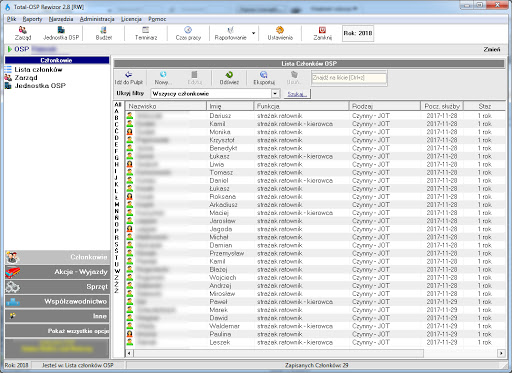
\includegraphics[width=\textwidth]{img/chapter2/total-osp.jpg}
    \caption{Interfejs użytkownika aplikacji TOTAL-OSP}
    \label{fig:TOTAL-OSP}
\end{figure}


Niestety interfejs aplikacji uchwycony na rys. \ref{fig:TOTAL-OSP} wygląda na bardzo przestarzały. Program został zaprojektowany na podobieństwo dawnego oprogramowania pakietów biurowych. Mimo sterylnego uporządkowania funkcjonalności, aplikacja zdaje się być nudnym i przytłaczającym narzędziem pracy.

Kolejną wadą rozwiązania, jest okoliczność, że z programu można korzystać jedynie na komputerach z zainstalowanym systemem operacyjnym z rodziny Microsoft Windows. Niweluje to możliwości wykorzystania narzędzia poprzez urządzenia mobilne, co czyni je o wiele mniej podręcznym, a przede wszystkim wolniejszym. Konsekwencją powyższych wad jest możliwość korzystania z aplikacji jedynie przy komputerze stacjonarnym znajdującym się w budynku jednostki OSP. 
Na plus, można wyróżnić możliwość instalacji oprogramowania na wielu komputerach w tej samej sieci LAN, w ramach jednej licencji oraz gotowy mechanizm tworzenia kopii zapasowych bazy danych. 


%%%%%%%%%%%%%%%%%%%%%%%%%%%%%%%%%%%%%%%%%%%%%%%%%%%%%%%%%%%%%%%%%%%%%%%%%%%%%%%%
\section{mOSP}
%%%%%%%%%%%%%%%%%%%%%%%%%%%%%%%%%%%%%%%%%%%%%%%%%%%%%%%%%%%%%%%%%%%%%%%%%%%%%%%%

Kolejne rozwiązanie zostało stworzone przez polską firmę MatSol. Według danych zamieszczonych na stronie produktu, w roku 2015 ponad 600 jednostek OSP wykorzystywało ich produkt, co świadczy o jego umiarkowanym sukcesie na rynku oprogramowania \cite{mOSP}.

mOSP jest konkurencyjną aplikacją, stworzoną w bardzo zbliżonym okresie do rozwiązania opisanego w sekcji 2.2. Poza mniej użytecznymi dodatkami, takimi jak moduł odpowiedzialny za organizację zawodów strażackich, posiada ona praktycznie te same funkcjonalności co TOTAL-OSP.

\begin{figure}
    \centering
    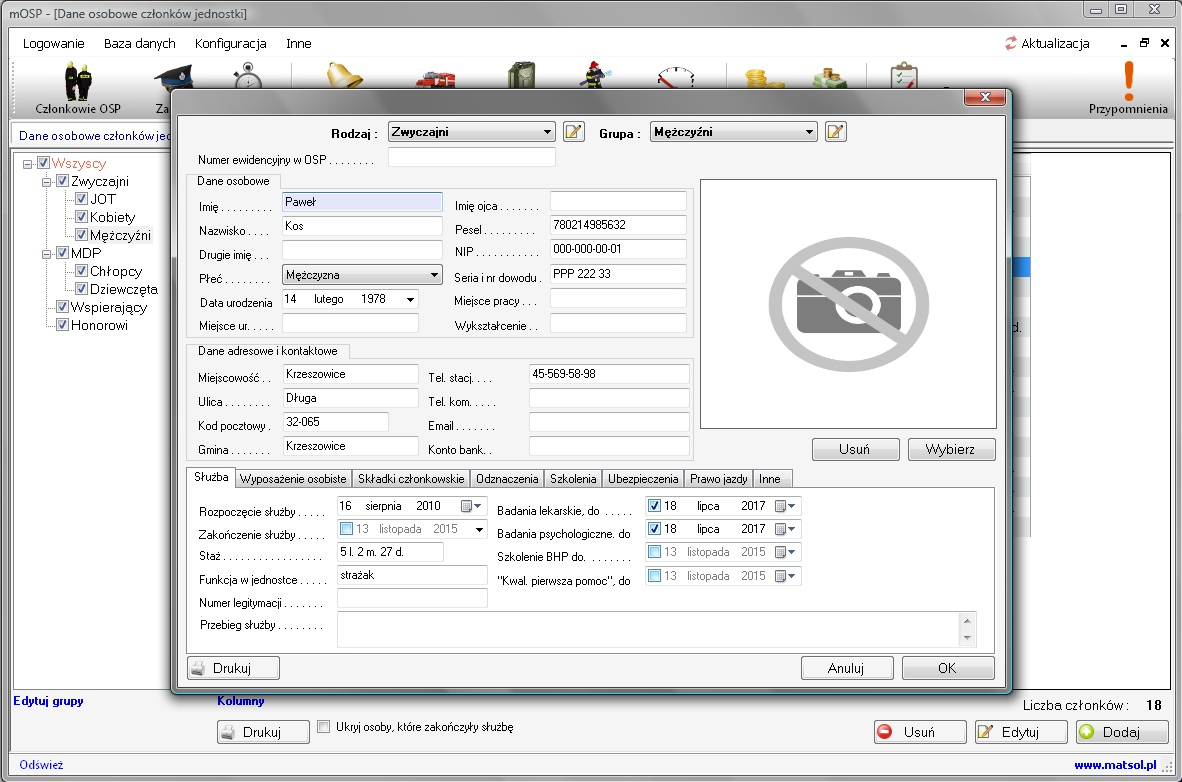
\includegraphics[width=\textwidth]{img/chapter2/m-osp.jpg}
    \caption{Interfejs użytkownika aplikacji mOSP}
    \label{fig:mOSP}
\end{figure}

Twórcy mOSP uczynili interfejs użytkownika programu podobnym do arkuszy kalkulacyjnych, w których najważniejszą rolę pełnią tabele (rys. \ref{fig:mOSP}). Zunifikowany interfejs odpłaca się bardziej intuicyjną obsługą oprogramowania. Niestety, mimo dużej sterylności widoków, program wydaje się być przestarzały i nieciekawy dla użytkownika.

Jedna licencja oprogramowania pozwala na skorzystanie z aplikacji na trzech komputerach, ale jedynie z systemem operacyjnym Windows. Analogicznie jak w przypadku opisanej powyżej aplikacji TOTAL-OSP brak jest możliwości wykorzystania narzędzia poprzez urządzenia mobilne do codziennej pracy w terenie. 

%%%%%%%%%%%%%%%%%%%%%%%%%%%%%%%%%%%%%%%%%%%%%%%%%%%%%%%%%%%%%%%%%%%%%%%%%%%%%%%%
\section{OSPiko}
%%%%%%%%%%%%%%%%%%%%%%%%%%%%%%%%%%%%%%%%%%%%%%%%%%%%%%%%%%%%%%%%%%%%%%%%%%%%%%%%

Ostatnim rozpatrywanym rozwiązaniem jest  OSPiko od przedsiębiorstwa TomPiko. Program zyskał uznanie wielu jednostek OSP, których opinie można przeczytać na stronie producenta \cite{OSPiko}.

OSPiko dubluje wszystkie najważniejsze funkcjonalności swoich poprzedników, rozbijając niektóre moduły na mniejsze. Każdy z modułów ewidencyjnych posiada również możliwość drukowania ujednoliconych i prostych raportów z działalności jednostki.

\begin{figure}
    \centering
    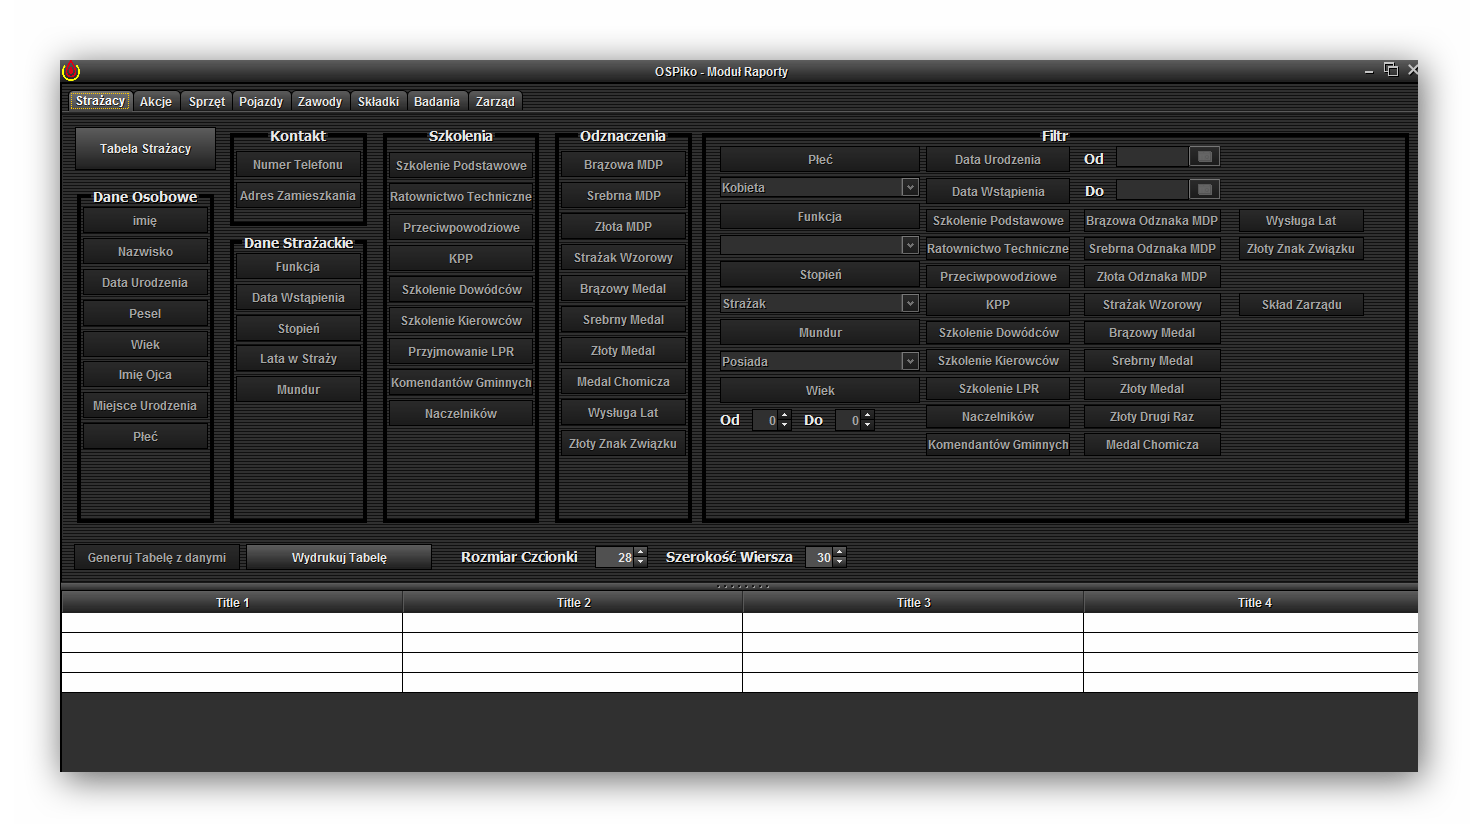
\includegraphics[width=\textwidth]{img/chapter2/ospiko.png}
    \caption{Interfejs użytkownika aplikacji OSPiko}
    \label{fig:OSPiko}
\end{figure}

Aplikacja wyróżnia się spośród pozostałych bardziej nowoczesnym interfejsem użytkownika i dobrą organizacją okien oraz formularzy (rys. \ref{fig:OSPiko}). Powyższe, czyni ją bardziej przyjazną użytkownikowi i sprawia, że korzystanie z niej wiąże się z większą satysfakcją.

Twórcy programu udostępniają możliwość kupna licencji przypisanej sprzętowo do jednego komputera lub wersji przenośnej, umożliwiającej korzystanie z oprogramowania na różnych stanowiskach, ale wyłącznie z zainstalowanym systemem operacyjnym Windows. Ogranicza to możliwość korzystania z aplikacji w terenie, podobnie jak w przypadku konkurencyjnych produktów.


%%%%%%%%%%%%%%%%%%%%%%%%%%%%%%%%%%%%%%%%%%%%%%%%%%%%%%%%%%%%%%%%%%%%%%%%%%%%%%%%
\section{Podsumowanie}
%%%%%%%%%%%%%%%%%%%%%%%%%%%%%%%%%%%%%%%%%%%%%%%%%%%%%%%%%%%%%%%%%%%%%%%%%%%%%%%%

Funkcjonujące na rynku, gotowe rozwiązania są bardzo funkcjonalnymi programami, które spełniają swoje zadania w dostatecznym stopniu. Niektóre z nich, poza prowadzeniem elektronicznego rejestru jednostki, udostępniają możliwość drukowania statystyk i dokumentów przydatnych w pracy OSP.

Jednakże, ich wspólną wadą pozostaje fakt uzależnienia od komputerów z systemem Windows oraz stosunkowo mało atrakcyjne interfejsy użytkownika. Zniechęca to część potencjalnych klientów oraz co gorsza uniemożliwia wykorzystanie popularnych urządzeń mobilnych. Rezygnacja z szybkiej interakcji z systemem, przy pomocy dostępnego pod ręką urządzenia, stanowi poważny problem. Rozwiązanie tego problemu stanowi kluczowy element niniejszej pracy.
